\documentclass[11pt,a4paper,landscape]{article}
\usepackage[margin=0.5in]{geometry}
\usepackage{booktabs}
\usepackage{array}
\usepackage{xcolor}
\usepackage{colortbl}
\usepackage{adjustbox}
\usepackage{multirow}
\usepackage{graphicx}
\usepackage{tikz}
\usepackage{fontspec}
\usepackage[default,scale=0.95]{opensans}

% Define ENBEL color scheme
\definecolor{enbelblue}{RGB}{0,83,155}
\definecolor{enbelorange}{RGB}{255,127,0}
\definecolor{enbelgreen}{RGB}{44,160,44}
\definecolor{enbelpurple}{RGB}{148,103,189}
\definecolor{enbelred}{RGB}{214,39,40}
\definecolor{enbelgray}{RGB}{140,140,140}
\definecolor{lightblue}{RGB}{230,240,250}
\definecolor{lightorange}{RGB}{255,245,235}
\definecolor{darkgray}{RGB}{80,80,80}

\pagestyle{empty}

\begin{document}

\begin{center}
{\LARGE \color{enbelblue}\textbf{Study Design \& Methodological Framework}}\\[0.5em]
{\large \color{darkgray}Comprehensive Urban Climate-Health Analysis}
\end{center}

\vspace{1em}

% Study Population Section
\begin{adjustbox}{width=\textwidth,center}
\renewcommand{\arraystretch}{1.8}
\begin{tabular}{@{}ll@{}}
\toprule
\rowcolor{enbelblue}
\multicolumn{2}{@{}l@{}}{\textcolor{white}{\textbf{\Large STUDY POPULATION}}} \\
\midrule
\rowcolor{lightblue}
\textbf{Location} & 
\begin{tikzpicture}[baseline=(current bounding box.center)]
\node[fill=white, rounded corners=2pt, inner sep=3pt] {Johannesburg, South Africa (Urban African cohort)};
\end{tikzpicture} \\
\textbf{Total Sample} & \textcolor{enbelorange}{\textbf{N = 18,205 participants}} \\
\rowcolor{lightblue}
\textbf{Study Design} & Cross-sectional with temporal lag structure (0-21 days) \\
\textbf{Climate Metrics} & Daily temperature \& apparent temperature measurements \\
\bottomrule
\end{tabular}
\end{adjustbox}

\vspace{1.5em}

% Biomarker Sample Sizes
\begin{adjustbox}{width=0.9\textwidth,center}
\renewcommand{\arraystretch}{1.5}
\begin{tabular}{@{}lllc@{}}
\toprule
\rowcolor{enbelorange}
\textcolor{white}{\textbf{Category}} & 
\textcolor{white}{\textbf{Biomarker}} & 
\textcolor{white}{\textbf{Sample Size}} & 
\textcolor{white}{\textbf{Statistical Power}} \\
\midrule
\rowcolor{lightorange}
\multirow{2}{*}{\textbf{Cardiovascular}} & Systolic Blood Pressure & 4,957 & 

\begin{tikzpicture}[baseline=(current bounding box.center)]
\fill[enbelgreen] (0,0) rectangle (2,0.3);
\node[right] at (2.1,0.15) {\small >0.99};
\end{tikzpicture} \\
& Diastolic Blood Pressure & 4,957 & 

\begin{tikzpicture}[baseline=(current bounding box.center)]
\fill[enbelgreen] (0,0) rectangle (2,0.3);
\node[right] at (2.1,0.15) {\small >0.99};
\end{tikzpicture} \\
\rowcolor{lightorange}
\multirow{2}{*}{\textbf{Metabolic}} & Fasting Glucose & 2,731 & 

\begin{tikzpicture}[baseline=(current bounding box.center)]
\fill[enbelgreen] (0,0) rectangle (2,0.3);
\node[right] at (2.1,0.15) {\small >0.99};
\end{tikzpicture} \\
& Total Cholesterol & 2,497 & 

\begin{tikzpicture}[baseline=(current bounding box.center)]
\fill[enbelorange] (0,0) rectangle (1.6,0.3);
\node[right] at (2.1,0.15) {\small 0.80-0.95};
\end{tikzpicture} \\
\rowcolor{lightorange}
\textbf{Immune} & CD4 Cell Count & 1,283 & 

\begin{tikzpicture}[baseline=(current bounding box.center)]
\fill[enbelorange] (0,0) rectangle (1.6,0.3);
\node[right] at (2.1,0.15) {\small 0.80-0.95};
\end{tikzpicture} \\
\bottomrule
\end{tabular}
\end{adjustbox}

\vspace{1.5em}

% Statistical Methods
\begin{adjustbox}{width=\textwidth,center}
\renewcommand{\arraystretch}{1.6}
\begin{tabular}{@{}l>{\raggedright\arraybackslash}p{10cm}@{}}
\toprule
\rowcolor{enbelpurple}
\multicolumn{2}{@{}l@{}}{\textcolor{white}{\textbf{\Large STATISTICAL METHODOLOGY}}} \\
\midrule
\textbf{Primary Analysis} & Pearson correlation for continuous climate-biomarker relationships \\
\rowcolor{lightblue}
\textbf{Confidence Intervals} & Bootstrap method (1,000 iterations) for 95\% CI estimation \\
\textbf{Significance Testing} & Permutation testing (10,000 permutations) for robust p-values \\
\rowcolor{lightblue}
\textbf{Multiple Testing} & Bonferroni correction ($\alpha$ = 0.0125) + FDR adjustment \\
\textbf{Lag Analysis} & Structured periods: 0, 1, 2, 3, 5, 7, 10, 14, \textcolor{enbelorange}{\textbf{21 days}} \\
\rowcolor{lightblue}
\textbf{Validation} & Distributed Lag Non-linear Models (DLNM) confirmation \\
\bottomrule
\end{tabular}
\end{adjustbox}

\vspace{1.5em}

\begin{center}
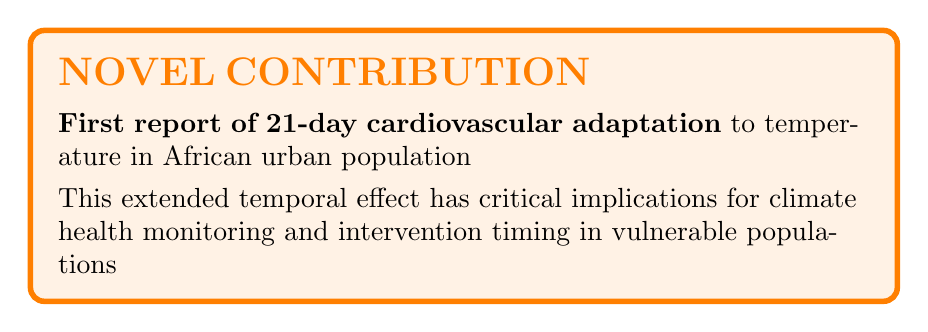
\begin{tikzpicture}
\node[draw=enbelorange, fill=enbelorange!10, rounded corners=5pt, inner sep=10pt, text width=0.85\textwidth, line width=2pt] {
\textbf{\Large \color{enbelorange}NOVEL CONTRIBUTION}\\[0.5em]
\textbf{First report of 21-day cardiovascular adaptation} to temperature in African urban population\\[0.3em]
This extended temporal effect has critical implications for climate health monitoring and intervention timing in vulnerable populations
};
\end{tikzpicture}
\end{center}

\end{document}